% report.tex
% main file for the project report.

\documentclass[a4paper,12pt,parskip=full]{scrreprt}

% german names
\usepackage{ngerman}
% utf-8
\usepackage{polyglossia}
\setmainlanguage[spelling=new]{german}
\usepackage{fontspec}
\usepackage{pdfpages}

% In order to remove scr warning
\usepackage{scrhack}

%Needed to wrap text around images, used for personas
\usepackage{wrapfig}

%Used to avoid page breaks with each chapter
\usepackage{etoolbox}
\makeatletter
\patchcmd{\chapter}{\if@openright\cleardoublepage\else\clearpage\fi}{}{}{}
\makeatother


% colored links
\usepackage{color}
\usepackage[colorlinks=true, citecolor=red] {hyperref}
\definecolor{grey}{rgb}{0.2,0.2,0.2}
\definecolor{orange}{rgb}{0.9,0.3,0}
\definecolor{turqoise}{rgb}{0,0.7,0.5}
\definecolor{listinggray}{gray}{0.9}
\definecolor{lbcolor}{rgb}{0.95,0.95,0.95}
\definecolor{Darkgreen}{rgb}{0.0,0.4,0.0}

% code listings
\usepackage{listings}
\renewcommand{\lstlistingname}{Code}
\lstset{
    backgroundcolor=\color{lbcolor},
    tabsize=4,
%   rulecolor=,
    language=[GNU]C++,
    basicstyle=\footnotesize\ttfamily,
    breaklines=true
    upquote=true,
    aboveskip={1.5\baselineskip},
    columns=fixed,
    showstringspaces=false,
    extendedchars=false,
    prebreak = \raisebox{0ex}[0ex][0ex]{\ensuremath{\hookleftarrow}},
    frame=single,
    numbers=left,
    showtabs=false,
    showspaces=false,
    showstringspaces=false,
    identifierstyle=\ttfamily,
    keywordstyle=\color{orange},
    commentstyle=\color[rgb]{0.026,0.112,0.095},
    stringstyle=\color[rgb]{0.627,0.126,0.941},
    numberstyle=\color[rgb]{0.205, 0.142, 0.73},
%   \lstdefinestyle{C++}{language=C++,style=numbers}’.
}
\lstset{
    backgroundcolor=\color{lbcolor},
    tabsize=4,
    language=C++,
    captionpos=b,
    tabsize=3,
    frame=lines,
    numbers=left,
    numberstyle=\tiny,
    numbersep=5pt,
    breaklines=true,
    showstringspaces=false,
    basicstyle=\footnotesize\ttfamily,breaklines=true
  %  identifierstyle=\color{magenta},
    keywordstyle=\color{orange},
    commentstyle=\color{turqoise},
    stringstyle=\color{Darkgreen}
}

\renewcaptionname{ngerman}{\figurename}{Abb.}
\renewcaptionname{ngerman}{\tablename}{Tab.}
% For adding the titelpage as a pdf
\usepackage{pdfpages}

% graphics
\usepackage{graphicx}
\graphicspath{{images/}}

% BibTex lib - used for citation
\usepackage{cite}

\usepackage[automark,headsepline,autooneside=false]{scrlayer-scrpage}
\clearpairofpagestyles{}
\ihead{\leftmark}
\chead{}
\ohead{\ifstr{\rightmark}{\leftmark}{}{\rightmark}}
%\ifoot{Bachelorthesis --- Tobias Kerst}
%\cfoot{}
\ofoot*{Seite\enspace\pagemark}
\pagestyle{scrheadings}
\setkomafont{pageheadfoot}{\normalfont}


% Increases spacing of footer line
\ModifyLayer[addvoffset=3ex]{scrheadings.foot.oneside}
\ModifyLayer[addvoffset=3ex]{plain.scrheadings.foot.oneside}

\usepackage{lipsum}

\setkomafont{disposition}{\normalfont\bfseries}

% for verbatiminput
\usepackage{verbatim}

% Nicely prints XeLaTeX
\usepackage{metalogo}

% Used for cross-referencing between different files
\usepackage{xr}

% not yet used
%\input{src/cmd}

\begin{document}

\titlehead{
	
\includegraphics[width=0.9\linewidth]{hska_logo}
}

\title{Systemnahes Programmieren}
\subtitle{Dokumentation zu Scanner \& Parser}
\author{%
	T. Kerst\\
	\textsc{47646}
	\and
	H. Klöppinger\\
	\textsc{47633}
	\and
	P. König\\
	\textsc{46910}
	\and
	K. Wolf\\
	\textsc{47308}
}
\date{Sommersemester 2017}
\publishers{
    \textbf{Dozent:} Prof.~Dr.~rer.~nat.~Oliver Waldhorst
}
\maketitle

\clearpage

\pagenumbering{Roman}
\phantomsection\addcontentsline{toc}{chapter}{Inhaltsverzeichnis}
\begingroup
\hypersetup{linkcolor=black}
\tableofcontents
\endgroup

\clearpage

\pagenumbering{arabic}

\chapter{Scanner}\label{chap:intro}

\section{Einleitung}
Aufgabe des Labors \textit{Systemnahes Programmieren} ist die Implementierung eines Compilers. Ein Compiler übersetzt ein Programm in einer vorgegebenen Sprache, in ein Programm in maschinennaher Sprache. Es sollen auch Fehler im Programmcode erkannt werden.

Die Aufgabe wurde in zwei Teilaufgaben aufgeteilt. Dieses Dokument befasst sich mit der ersten Teilaufgabe, der Implementierung eines Scanners.
Dabei handelt es sich um eine lexikalische Analyse, welche das vorgegebene Programm in Tokens, also ihre Grundsymbole, zerlegt.

Die Menge aller gültigen Zeichen und Bezeichner einer Programmiersprache ist üblicherweise eine reguläre Sprache.

Die gültigen Zeichen lauten wie folgt:
\begin{verbatim}
digit ::= 0 | 1 | 2 | 3 | 4 | 5 | 6 | 7 | 8 | 9
letter ::= A | B | C | … | Z | a | b | … | z
sign… ::= + | - | : | * | < | > | = | := | =:= | ! | && | ; | ( | ) | { | } | [ | ]
integer ::= digit digit*
identifier ::= letter (letter | digit)*
if ::= if | IF
while ::= while | WHILE
\end{verbatim}

Die gültigen Symbole bilden die reguläre Sprache
\begin{verbatim}
L( sign+ | … | sign] | integer | identifier | if | while)
\end{verbatim}

Zu dieser Sprache wird ein Automat erstellt. Dieser akzeptiert die Sprache und befindet sich in einem Finalzustand, wenn ein Wort akzeptiert wird, oder in einem Nicht-Endzustand, wird ein Wort nicht akzeptiert.

Erkannte Identifier werden in einer Symboltabelle gespeichert. Das Token enthält neben einem Verweis darauf auch die Informationen Zeile, Spalte, Typ. Sollten Symbole außerhalb der Menge der gültigen Zeichen oder Bezeichner gefunden werden, wird ein Fehlertoken erstellt.


\subsection{Voraussetzungen}
Um unser Projekt korrekt kompilieren zu können, sind einige Programme notwendig, die an dieser Stelle genannt werden sollen.
\begin{itemize}
  \item Gcc
  \item Make
  \item CMake (Version >= \textsc{3.5})
  \item Git
\end{itemize}

Möchte man diese Dokumentation generieren, benötigt man zudem
\begin{itemize}
  \item XeLaTeX
  \item BibTeX
  \item Python3
\end{itemize}
Das gesamte Projekt wurde mit Linux Mint 18 (Mate) getestet. Da eine Anforderung war, dass das Projekt mit Eclipse eingesetzt werden soll, haben wir beschlossen Eclipse Neon in der Version 4.6.3 zu nutzen, welches das Eclipse CDT Plugin in der Version 9.2.1 zur Entwicklung von C++ Programmen einsetzt.

Erstellen eines Projekts
Um das Projekt korrekt in Eclipse zu importieren, muss das Projekt zuerst geladen werden. Wir haben uns dazu entschieden, Github als Host unserers Git Repositories zu nutzen.

Das Projekt kann man wie folgt laden:

\begin{lstlisting}[language=bash,numbers=none]
git clone https://github.com/TobsCore/sysprog.git
\end{lstlisting}

Man erkennt, dass ein neues Verzeichnis mit dem Namen \texttt{sysprog/} erstellt wurde. Dies ist unser Projekt-Verzeichnis. Wie das Projekt organisiert ist, wird genauer in~\ref{sec:orga_code} genauer beleuchtet.

Es handelt sich bei uns um ein \textit{CMake Projekt}, was man unter anderem daran erkennt, dass sich im Hauptverzeichnis die Datei \texttt{CMakeLists.txt} befindet. Diese Datei wird dazu genutzt, dass alle Programmteile korrekt gelinkt werden und man kann dort verschiedene \textit{Compile Targets} definieren. Was dies bedeutet, werden wir sehen, wenn das Projekt erfolgreich in Eclipse importiert wurde.

Da Eclipse jedoch nicht mit CMake Projekten umgehen kann, kann man sich ein Eclipse Projekt durch CMake generieren lassen. Um diesen Schritt zu vereinfachen, haben wir ein kleines Script geschrieben, welches sich im \texttt{sysprog/} Verzeichnis befindet und dort ausgeführt werden kann.

\lstinputlisting[language=bash,numbers=none,caption=Das Init Eclipse Script]{../init_eclipse.sh}

An dieser Stelle sei anzumerken, dass sich in unserem Projekt 2 unterschiedlicheCMakeLists.txt Dateien befinden.
\begin{verbatim}
sysprog/CMakeLists.txt
sysprog/src/CMakeLists.txt
\end{verbatim}

Diese Dateien haben beinahe den selben Inhalt, was den Grund hat, dass wir das Programm auch unter MacOS mit CLion entwickeln wollten und Eclipse nicht damit umgehen kann, dass der Ordner \texttt{cmake-build-debug/}, in den die Executables geschrieben werden im Quellcodeverzeichnis liegt. Die \texttt{CMakeLists.txt} Datei, die zur Generierung des Eclipse Projekts genutzt wird, liegt also in \texttt{
sysprog/src/CMakeLists.txt}.

\subsection{Generierung des Eclipse Projekts}
Es wurde ja bereits beschrieben, das das Projekt in ein Eclipse Projekt umwandelt. Dieses Script kann man einfach per

\begin{lstlisting}[language=bash,numbers=none]
./init_eclipse.sh
\end{lstlisting}

aufrufen. Hierbei wird der Ordner \texttt{cmake-build-debug/} generiert, in den dann die Executables nach erfolgreichem Kompilieren landen.

Das Projekt kann nun in Eclipse eingebunden werden. Hierzu wählt man \textit{File} -> \textit{Import}. Unter \textit{General} wählt man dann den Eintrag \textit{Existing Projects into Workspace}.
Bei dem Punkt \textit{Select root directory} wählt man dann den gerade generierten Ordner \texttt{sysprog/cmake-build-debug/}.

Das Ganze sollte dann wie auf Bild~\ref{fig:import_project} aussehen. Wichtig ist hierbei, dass die Option \textit{Copy projects into workspace} deaktiviert ist.

\begin{figure}[!htb]
    \centering
      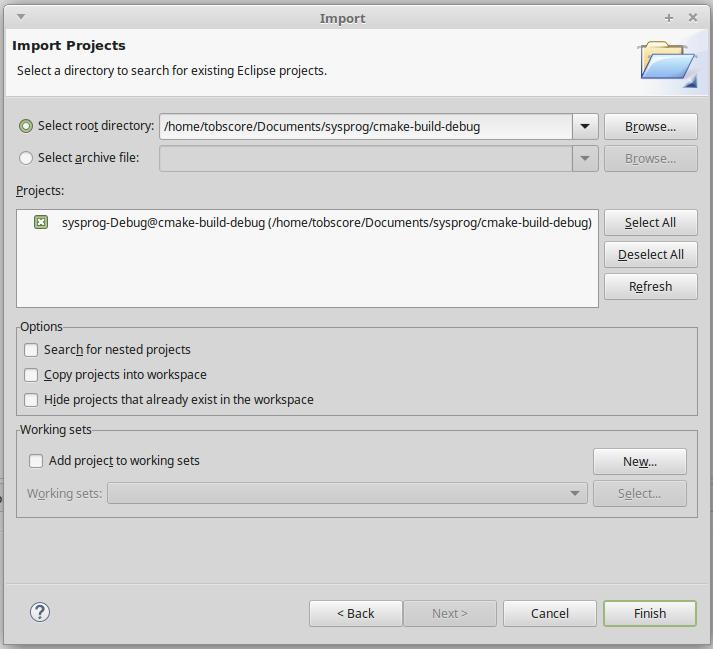
\includegraphics[width=0.6\linewidth]{Import_Project.jpg}
    \caption{Import Dialog}\label{fig:import_project}
\end{figure}

Durch das Klicken auf \textit{Finish} sollte das Projekt dann korrekt eingebunden sein.
\clearpage

\setlength{\intextsep}{-20pt}%
\begin{wrapfigure}{r}{0.35\textwidth}
  \centering
    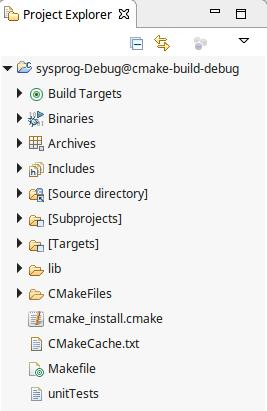
\includegraphics[width=0.32\textwidth]{Project_Structure.jpg}
    \caption{Die Projekt\-struktur in Eclipse}\label{fig:project_structure}
\end{wrapfigure}

In Bild~\ref{fig:project_structure} kann man dann sehen, wie die Projektstruktur in Eclipse aussieht.

Unter \textit{Build Targets} kann man dann den Eintrag \texttt{[exe] sysprogMain} auswählen und bauen, indem man einen Rechtsklick machet und \textit{Build Target} auswählt. Möchte man die Unit Tests laufen lassen, so kann man diese über \texttt{[exe] unitTests} kompilieren. Im Project Explorer wird dann unter Binaries das ausführbare Programm erstelllt.


Ausführen lassen sich die Programme direkt aus Eclipse über einen Rechtsklick auf eines der Binaries und danach durch Auswählen von \textit{Run As} -> \textit{Local C/C++ Application}.

Wie man erkennen kann, werden die Tests ausgeführt und in der Konsole innerhalb von Eclipse ausgegeben. Man kann dann auch Programmparameter für das Binary festlegen und somit auch das Hauptprogramm korrekt starten.

\subsection{Projekt ohne Eclipse kompilieren}
Möchte man das Projekt zum Laufen bringen, ohne sich an Eclipse binden zu müssen, so reicht es ein neues Verzeichnis zu erstellen, in dem dann durch CMake ein Makefile generiert wird. Dieses kann man dann sehr einfach ansprechen um BuildTargets zu bauen. Dies wird wie folgt gemacht.

\begin{lstlisting}[language=bash,numbers=none]
mkdir cmake-build-debug
cd cmake-build-debug
cmake ..
make all
\end{lstlisting}

Es lassen sich die Build Targets \texttt{sysprogMain} und \texttt{unitTests} auch gezielt bauen, durch den Aufruf

\begin{lstlisting}[language=bash,numbers=none]
make sysprogMain
make unitTests
\end{lstlisting}

In diesem Ordner werden dann die Binaries gebaut, die dann ausgeführt werden können.
\begin{lstlisting}[language=bash,numbers=none]
make unitTests
./unitTests
\end{lstlisting}

\subsection{Organisation des Codes}\label{sec:orga_code}
Wenn man das Repository herunter geladen hat, so findet man 2 Verzeichnisse. In \texttt{Documentation/} befindet sich diese Dokumentation, die mit \XeLaTeX\ erstellt wurde. Hat man \texttt{Python3} installiert, so kann man diese Dokumentation ganz einfach über \texttt{make} generieren lassen.

Das \texttt{src/} Verzeichnis enthält den Code für unser Programm, die Tests und alles was man zum erfolgreichen Bauen benötigt.

In dem \texttt{lib/} Verzeichnis befindet sich die \textit{Google Test} Bibliothek, welche wir verwendet haben um unsere Unit Tests zu schreiben.

Die Unit-Tests sind im Verzeichnis \texttt{test/}, wobei dort einige Testdateien im Verzeichnis \texttt{testData/} liegen. Ausführlichere Informationen zu den Unit-Tests gibt es bei~\ref{sec:UnitTests}.

Der eigentlich Source Code liegt dann unter \texttt{main/}.

\section{Buffer}
Der Buffer hat die Aufgabe eine Textdatei einzulesen und deren Inhalt zu speichern.

Um dies zu realisieren werden zwei Speicherblöcke mit der gleichen, festen Größe erstellt. Diese Speicherblöcke speichern dann den Inhalt der einzulesenden Textdatei. Die Speicherblöcke werden dazu abwechselnd gefüllt. Die Notwendigkeit dafür resultiert aus der Anforderung, gegebenenfalls ein Zeichen zurückzugehen. Ein Speicherblock würde die dieser Anforderung nicht gerecht, da dieser beim Überlaufen überschrieben werden würde, damit vorherige Zeichen nicht mehr vorhanden sind und entsprechend auch nicht mehr gelesen werden können.

Mit der Funktion \texttt{getChar()} des Buffers wird das nächste Zeichen geholt. Wird das letzte Zeichen eines Speicherblocks gelesen wird die Methode \texttt{fillBuffer()} aufgerufen, die den jeweils anderen Speicherblock, in dem man sich zurzeit nicht befindet, befüllt. Dann wird der neu befüllte Speicherblock zum aktuellen gemacht.

Die Methode \texttt{ungetChar()} dient dazu Zeichen gegebenenfalls zurückzugehen, damit ein Zeichen nach Tokenerstellung erneut gelesen werden muss. Sofern diese Aktion im selben Speicherblock stattfindet wird ganz simpel ein Index zurückgegangen, sollte das aktuelle Zeichen am Anfang einer der Speicherblöcke stehen, wird der aktuelle Block gewechselt, und die Indexposition neu berechnet.

Wird der Buffer nicht mehr benötigt, wird auch die einzulesende Datei geschlossen.

\section{Symboltabelle}
Die Symboltabelle speichert für alle Identifier und Schlüsselworte eine Token-Info-Container. Dies ist relevant, da sich so gleiche Lexeme, die als Identifier erkannt werden, denselben Info-Container teilen. Um ein performantes überprüfen, ob ein Lexem bereits einen Info-Container besitzt, zu ermöglichen, ist die Symboltabelle als HashMap implementiert. Kollisionsauflösung wurde durch Verkettung realisiert.

Soll ein Lexem eingefügt werden, muss für jedes ein Info-Container mit entsprechendem Typ erstellt werden.
Soll ein noch nicht vorhandener Container in die Liste eingetragen werden, wird zunächst der Hashwert des Lexems berechnet. Dieser gibt an, in welcher der verketteten Listen das Lexem abgelegt wird bzw.~gesucht werden muss.

Sollte noch keine Liste vorhanden sein, wird diese erstellt und ein Hashwert generiert, der das erneute auffinden realisiert. Dieser wird zurückgegeben.

Ist diese Liste leer, kann der Container einfach eingefügt werden. Enthält diese aber bereits Elemente, wird überprüft ob es für das Lexem bereits ein Container in ihr vorhanden ist. Sollte dieser Fall nicht eintreten wird der neue Container an die Liste angehängt und der generierte Hashwert zurückgegeben. Sollte aber bereits ein passender Container gefunden werden, wird dessen Hashwert zurückgegeben.

\begin{figure}[!htb]
    \centering
      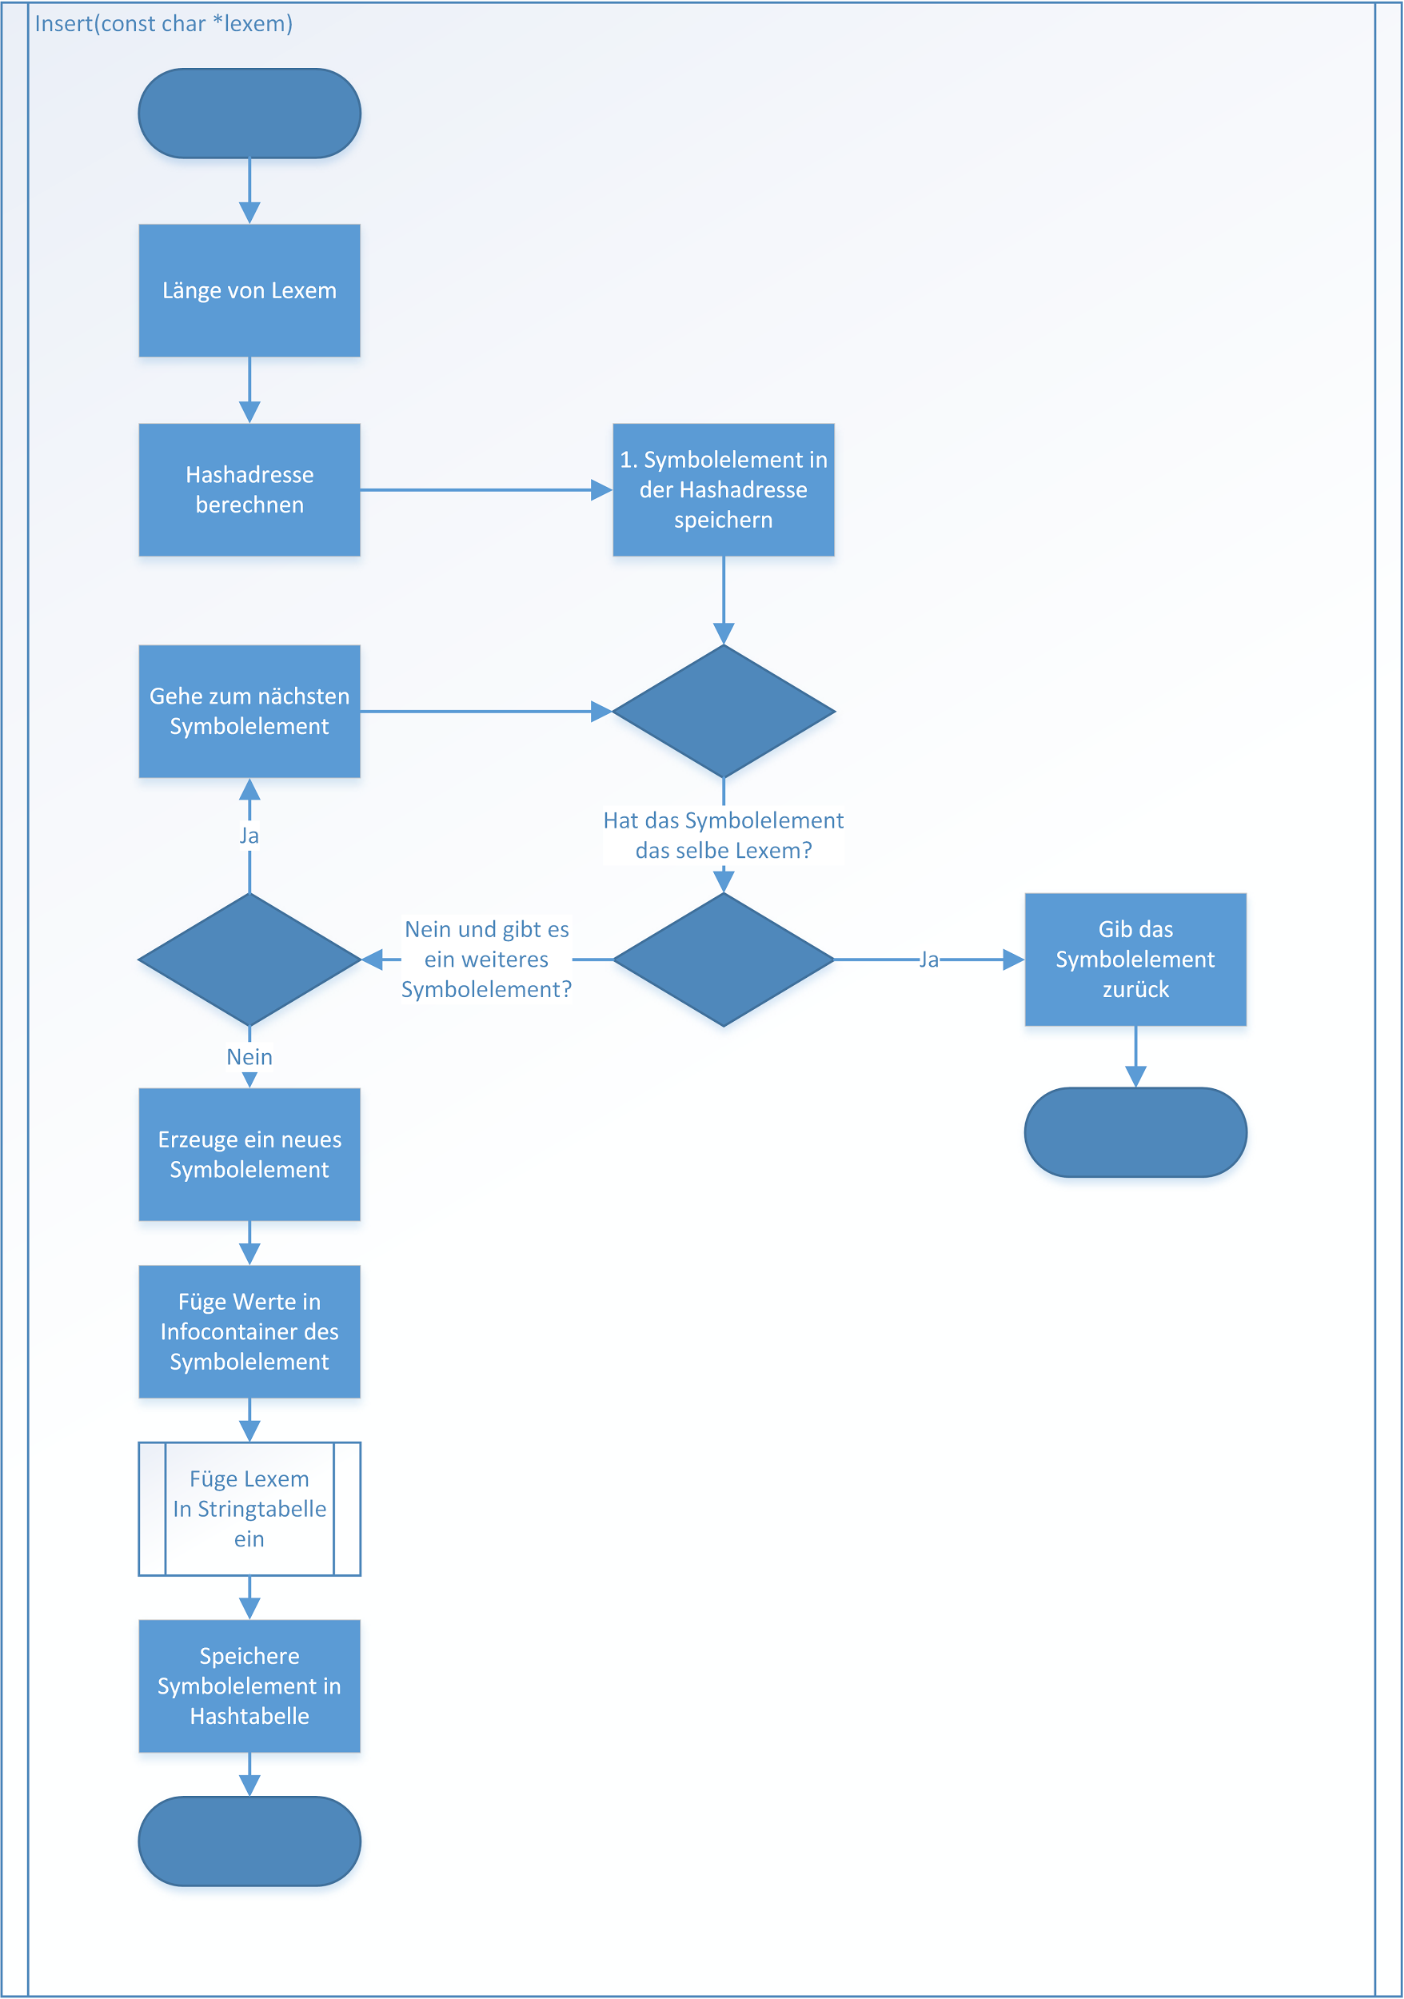
\includegraphics[width=0.6\linewidth]{Symboltabelle.png}
    \caption{Aktivitätsdiagramm Symboltabelle}\label{fig:symboltabelle}
\end{figure}

\section{Stringtabelle}
Die Stringtabelle speichert alle Lexeme als String ab.
Das Vorgehen sieht dabei wie folgt aus: Beginnend mit dem ersten Element des Lexemstrings werden eben diese der Reihe nach in die Stringtabelle eingefügt. Die Position, an der Eingefügt werden soll,  ist über einen Pointer auf die Stringtable bekannt. Dies geschieht solange, bis das letzte Element des Lexemstrings erreicht wurde. Dadurch wird die Länge des Lexems bestimmt.

Nun muss abgefragt werden ob das Lexem größer ist, als der bereitgestellte Stringspeicher (\texttt{int stringMemorySize = 1024}). Ist dies der Fall, wird Null zurückgegeben und es kommt zu einem Fehlerfall. Sollte der bereitgestellte Speicher aber ausreichen, wird der String entsprechend abgelegt.

Der restliche Speicher wird dann für ein neues Element bereitgestellt und der Index in der Stringtabelle um die entsprechende Länge des Lexems angepasst, um ein neu gelesenes Lexem zu speichern. Sollte der restliche Speicher nicht für ein weiteres Lexem ausreichen, wird eine neue Stringtable erstellt, welche mit der vorherigen verknüpft werden muss.

\begin{figure}[!htb]
    \centering
      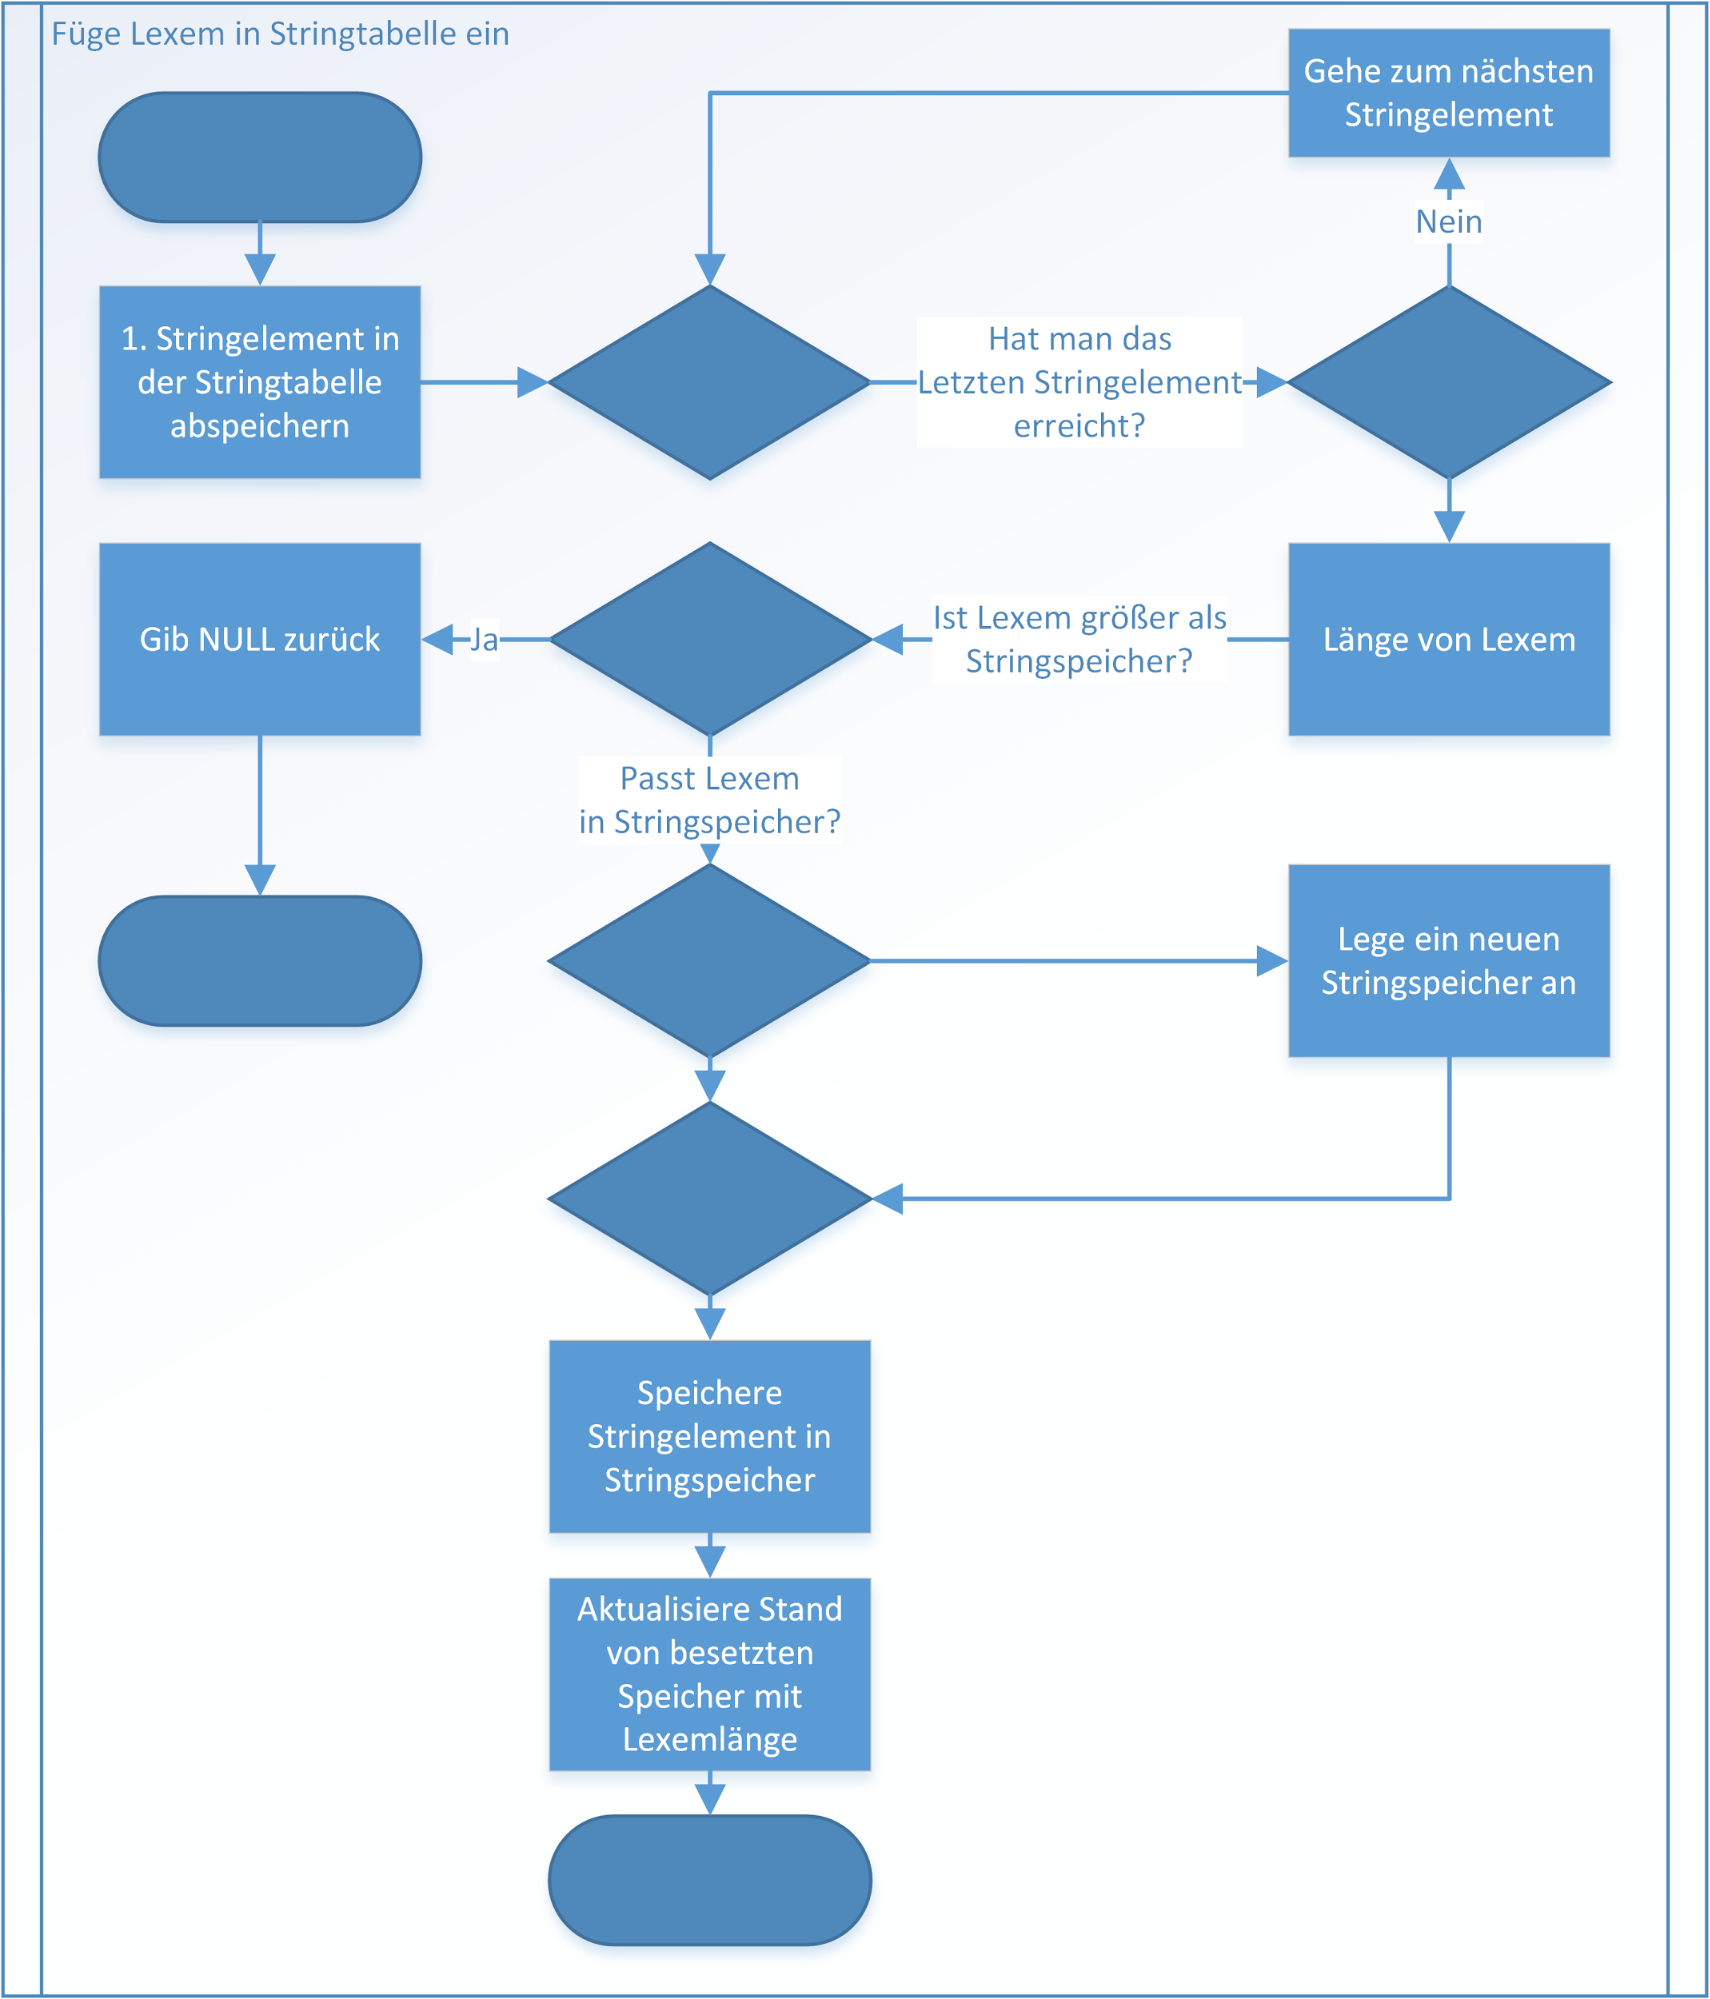
\includegraphics[width=0.6\linewidth]{Stringtabelle.png}
    \caption{Aktivitätsdiagramm Stringtabelle}\label{fig:stringtabelle}
\end{figure}

\section{Unit-Testing}\label{sec:UnitTests}
Damit das Programm auch verlässlich funktioniert, haben wir uns dafür entschieden, Unit Tests einzusetzten, anstatt händisch verschiedene Dateien zu testen. Somit können wir garantieren, dass gewisse Dinge funktionieren und diese Unit Tests dienen gleichzeitig auch dem \textit{Regression Testing}, da das Verändern von Code ohne weiteres problemlos möglich ist. Somit war es einigermaßen einfach, den Code zu verbessern und \textit{Refactoring} zu betreiben.

Wir setzen das Google Test\footnote{\url{https://github.com/google/googletest}} Framework ein, was es ermöglicht, Tests in Gruppen einzusortieren, einzelne Tests auszuschalten und auch Ausgabe-Dateien zu schreiben, die von anderen Tools dann gelesen und analysiert werden können. Es gibt die Möglichkeit Objekte ein einziges Mal zu erstellen und danach wieder zu benutzen.

\begin{lstlisting}[language=C++, caption=Unit Test mit wiederverwendbarem Objekt]
using testing::Eq;

namespace {
  class AutomatTest : public testing::Test {
  public:
      Automat testAutomat;
  };
}

TEST_F(AutomatTest, IntegerAddition) {
  ASSERT_EQ(testAutomat.checkExpression('1'), NEXTCHAR);
}
\end{lstlisting}

In dem Beispielcode erkennt man, dass das Objekt \texttt{testAutomat} in dem TestFall \emph{IntegerAddition} verwendet werden kann, ohne es in dem Testfall zu deklarieren. Hierzu dient die \texttt{TEST\_F} Notation. Im Normalfall konnte man jedoch einen einfachen Test wie folgt schreiben:

\begin{lstlisting}[language=C++, caption=Einfacher Unit Test]
TEST(BufferTest, LongFileWithLoopSwitchOnce) {
  char const *testFile = "../src/test/testData/LongFile.txt";
  Buffer* buffer = new Buffer(testFile);

  // With a buffer size of 1024, the buffer should be switched at least once
  for (int i = 0; i < 1050; i++) {
      char charVal = (i % 10) + 48;
      ASSERT_EQ(charVal, buffer->getChar());
  }
  delete buffer;
}
\end{lstlisting}

Würde man den Test mit dem Namen \emph{LongFileWithLoopSwitchOnce} in \emph{DISABLED\-\_LongFileWithLoopSwitchOnce} umbenennen, so würde das Testing Framework diesen Test ignorieren, was besonders im Zusammenspiel mit unserem Continuous Integration System \textit{TravisCI} (mehr dazu unter~\ref{sec:ContinousIntegration}) sehr praktisch war, weil man so Testfälle vorbereiten konnte, die jedoch noch nicht direkt korrekt liefen, ohne, dass der Build fehlschlägt.

\subsection{Was getestet wurde}
Die Unit Tests konnten sehr gut dazu benutzt werden, um Randfälle zu betrachten. So konnten wir die einzelnen Komponenten (Buffer, Scanner) z.B. darauf testen, wie sie mit leeren (Eingabe-) Dateien umgehen. Zudem konnte das Programm so inkrementell entwickelt werden. Hier ist der Buffer ein gutes Beispiel.

Zuerst wurde ermöglicht, dass der Buffer nur einzelne Zeichen einlesen kann, dann wurden so viele Zeichen eingelesen, dass der 2. Buffer genutzt werden musste. Dann so viele, dass der 1. Teil des Buffers erneut genutzt werden musste. Und im Anschluss wurde dann die Funktionalität von \texttt{unhgetchar()} implementiert, welche dann auf die Bufferwechsel angepasst wurde. Dadurch konnte dann auch sichergestellt werden, dass das Zeichen \texttt{=:=} korrekt behandelt werden kann, auch wenn es fehlerhaft an einem Bufferwechsel-Ort steht.

Wir haben in den Unit Tests zudem überlange Integer und Identifier getestet, um so zu gewährleisten, dass das Programm nicht unerwartet crashed. Zum Zeitpunkt haben wir knapp 100 Unit Tests.

\section{Continuous Integration}\label{sec:ContinousIntegration}
Um die Lauffähigkeit unseres Programms zu gewährleisten, setzen wir \texttt{TravisCI} ein, ein Tool mit dem man Continuous Integration umsetzen kann und das sehr gut mit Github Repositories zusammenarbeitet. Dem Repository wird eine \texttt{.travis.yml} Datei hinzugefügt, die konfiguriert, wie das Projekt gebaut werden soll und welche Schritte zusätzlich ausgeführt werden sollen.

Wir haben uns dafür entschieden, das Projekt für MacOS und für Linux zu testen. Hierzu wählen wir sowohl \texttt{clang}, als auch \texttt{gcc}, da wir somit die wichtigsten Compiler abdecken. Das Programm wird dann von Travis für diese 4 Konfigurationen gebaut und jedes Mal werden alle Unit-Tests ausgeführt, sodass gewährleistet ist, dass nichts schief geht. Sollte es jedoch zu einem Fehler kommen, so wird derjenige, der den Commit gemacht hat, per E-Mail über diesen Fehlschlag benachrichtigt.

\section{Programmausführung}
Wenn man das Programm mit make kompiliert, bekommt man eine ausführbare Datei (auch \textit{Executable}) mit dem Namen \texttt{scanner}. Diese kann man dann im Terminal einfach ausführen:

\begin{lstlisting}[language=bash,numbers=none]
>./scanner
\end{lstlisting}

Hierbei bekommt man dann die Ausgabe

\begin{lstlisting}[language=bash,numbers=none]
>./scanner
usage:
scanner <inputfile> <outputfile>
\end{lstlisting}

Diese Ausgabe bekommt man, damit man weiß, dass man zusätzlich auch noch die Ein- und Ausgabedatei mit angeben muss. Wenn dies gemacht wird, so wird die Eingabedatei gelesen und in die verschiedenen Token aufgeteilt. Zum Schluss wird die Ausgabedatei geschrieben.

\begin{lstlisting}[language=bash,numbers=none]
>./scanner EingabeKorrekt.txt out.txt
./scanner ../src/test/testData/Programm.txt out.txt
Running...
Finished!
Output written to <out.txt>
\end{lstlisting}

Sollte es zu Fehlern kommen, so werden diese direkt ausgegeben.
\begin{lstlisting}[language=bash,numbers=none]
>./scanner ./EingabeMitFehler.txt out.txt
Running...
Error Found! Line:   2 Column:   1  Info: Integer out of range
Finished!
Output written to <out.txt>
\end{lstlisting}

Hierbei wird der Fehler zudem farblich hervorgehoben, sodass der Nutzer des Programms definitiv mitbekommt, dass es zu einem Fehler gekommen ist. Das Programm bricht jedoch nicht ab, sondern versucht weiter die Eingabedatei in Token zu unterteilen.

Bei dem oben gezeigten Fehler, wird zudem die Ursache für den Fehler mit angegeben, dies ist jedoch nicht immer möglich und ist somit von dem Fehlertyp abhängig.

%\chapter{Parser}
\label{chap:chap2}

\lipsum[1]{}

\section{Beispiel für ein Bild}
\label{sec:objekthierarchie}

\lipsum[2]{}


% \clearpage
\phantomsection\addcontentsline{toc}{chapter}{Literaturverzeichnis}
\bibliography{sources}
\bibliographystyle{ieeetr}
\clearpage

\phantomsection\addcontentsline{toc}{chapter}{Abbildungsverzeichnis}
\listoffigures
\clearpage

\phantomsection\addcontentsline{toc}{chapter}{Quellcodeverzeichnis}
\lstlistoflistings\clearpage

\end{document}
